\label{chapter4}

\chapter{Results and Discussion}
\section{Introduction}
This chapter consist of two main parts namely results and discussion. It presents the findings and interpretations of the results. It also discusses the findings in context with literature. The findings are visualized using graphs.

\section{Results}	

\begin{figure}[!ht]
	\centering
	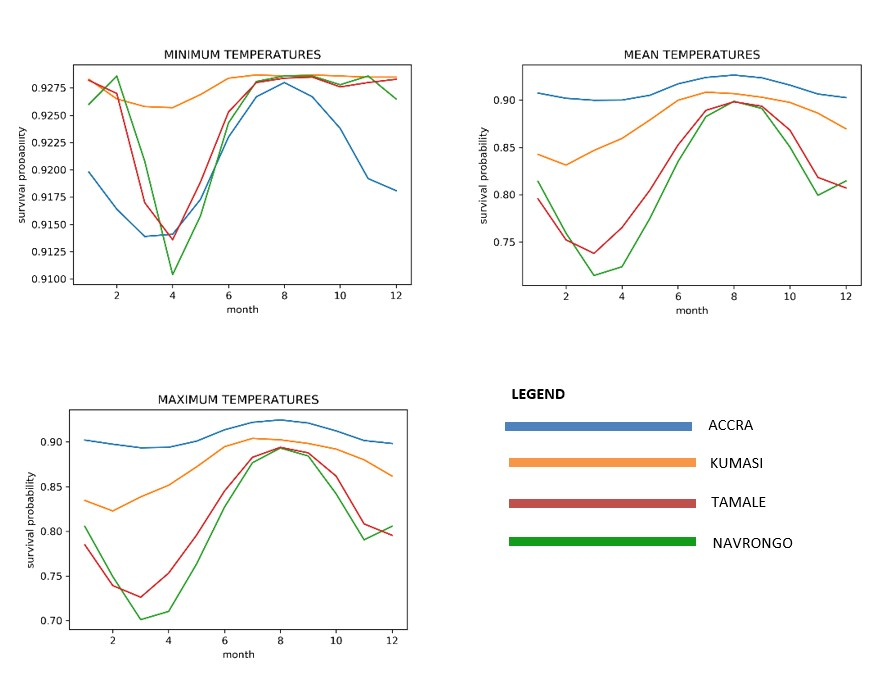
\includegraphics[scale=0.7]{survival-prob.jpg}
	\caption{Monthly Survival Propability of the malaria vector}
	\label{fig4.1}
\end{figure}
\noindent Figure \ref{fig4.1} shows the trend of the monthly survival probability as a function of temperature across the various agro-ecological zones. The graph shows that the survival probability was higher at both coastal and forest zones than the northern zone. Also, the survival probability was higher  between the month of June and October and lower between March and May across all zones.

 
\begin{figure}[!ht]
	\centering
	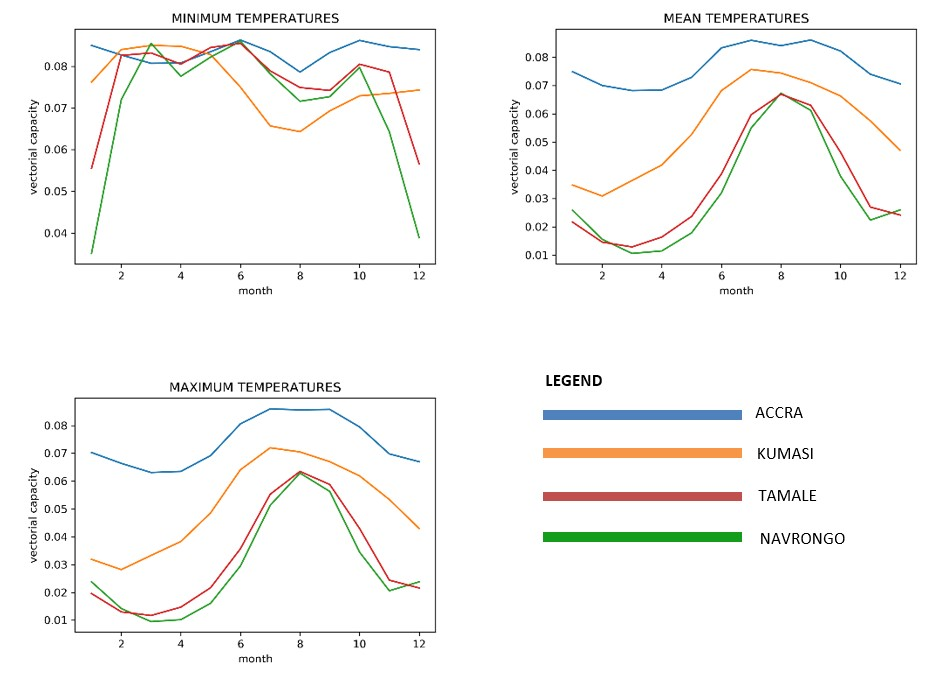
\includegraphics[scale=0.7]{vectorial-capa.jpg}
	\caption{Monthly Vectorial Capacity of the malaria vector}
	\label{fig4.2}
\end{figure}

\noindent Figure \ref{fig4.2} shows the trend of the vectorial capacity as a function of temperature across the various agro-ecological zones. The graph shows that the vectorial capacity was higher at both coastal and forest zones than northern zone. Also the vectorial capacity was higher between the month of June and October and lower between March and May across all zones.


\section{Discussion}
The goal of the study was to assess the influence of climate change on malaria vectorial capacity across Ghana's agro-ecological zones. The study discovered that in places with optimum temperatures, both vectorial capacity and survival probability were generally high. The vectorial capacity as well as the ability of malaria vectors to survive were also found to be low in places where temperatures were higher.
The vectorial capacity and survival probability in the Northern zone were higher during the wet season but very low during the dry season. For areas found in both coastal and forest zone, the vectorial capacity as well as the survival probability of malaria vectors were higher throughout the year. 
Malaria vectors' survival and vectorial capacity are both reduced as temperature rises. The vectorial capacity and survival probability were both higher between July and September, with August having the biggest peak across all agro-ecological zones. From February to April, however, both vectorial capacity and survival probability were low in all agro-ecological zones. The results for the vectorial capacity were expected because the northern zone of the
country has a very high temperatures which provides unfavorable conditions for the transmission of malaria. However, at the coastal and the forest zones, there is an increase in malaria transmission due to the fact that these areas provide optimum temperatures for malaria vectors. As a matter of fact, the population of malaria vectors are more in the coastal and the forest zones as compared to the other zones.\\

\noindent The study therefore showed that temperature seasonality have influence on seasonal changes in survival probability and the vectorial capacity of malaria vectors as well as determined how the survival probability and the vectorial capacity of malaria vectors differ as a function of climate and environment in Ghana.








